\section{What Pathways are important?}

\subsection{Damage Repair}
\begin{frame}[c]{Senescent Cell Effects}
    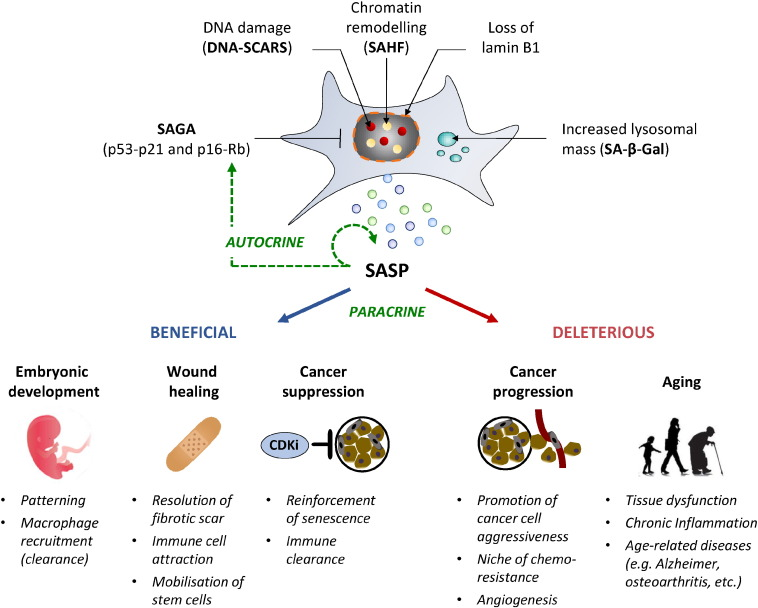
\includegraphics[height=0.85\textheight]{sasp_effects} \\
    Source: \cite{malaquin2016keeping}
\end{frame}


% \begin{frame}[c]{DNA Damage Response}
%     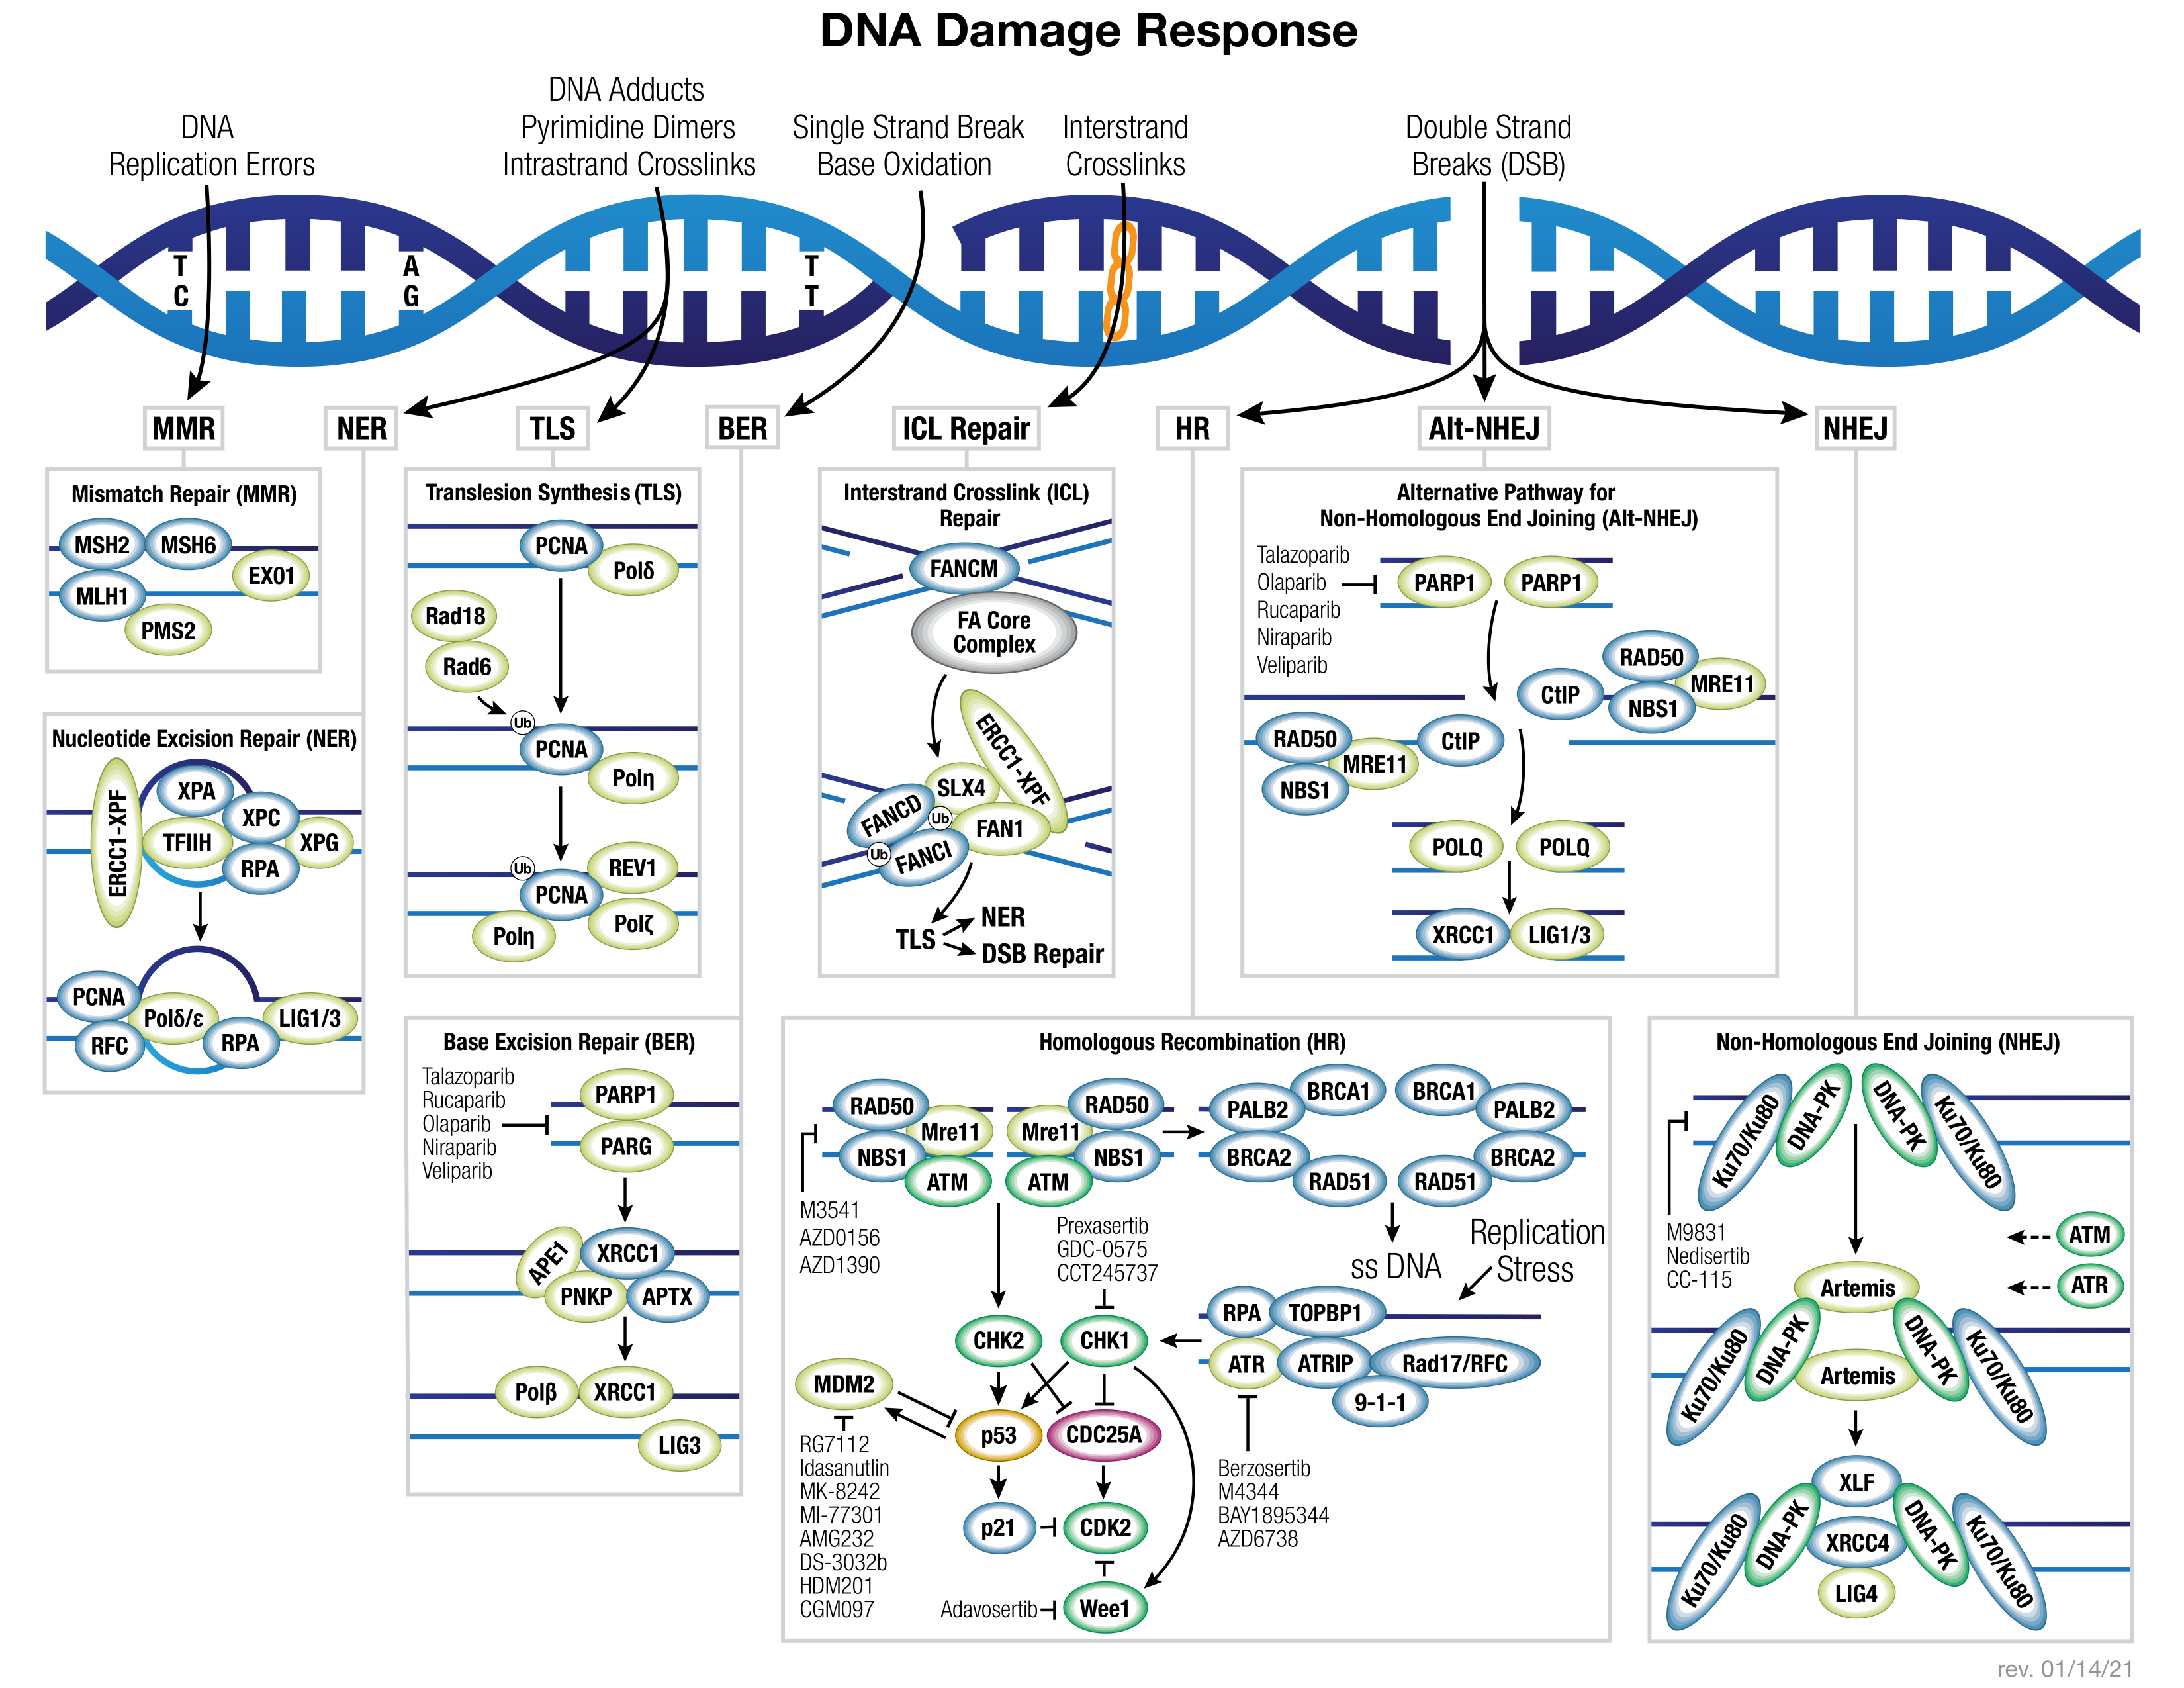
\includegraphics[height=0.85\textheight]{DNA-Damage-Response_2} \\
%     Source: \cite{DNADamag68:online}
%     \pnote{Not sure what I want to say here?}
% \end{frame}


\subsection{Calorie Restriction}

\begin{frame}[c]{Calorie Restriction Pathways}
    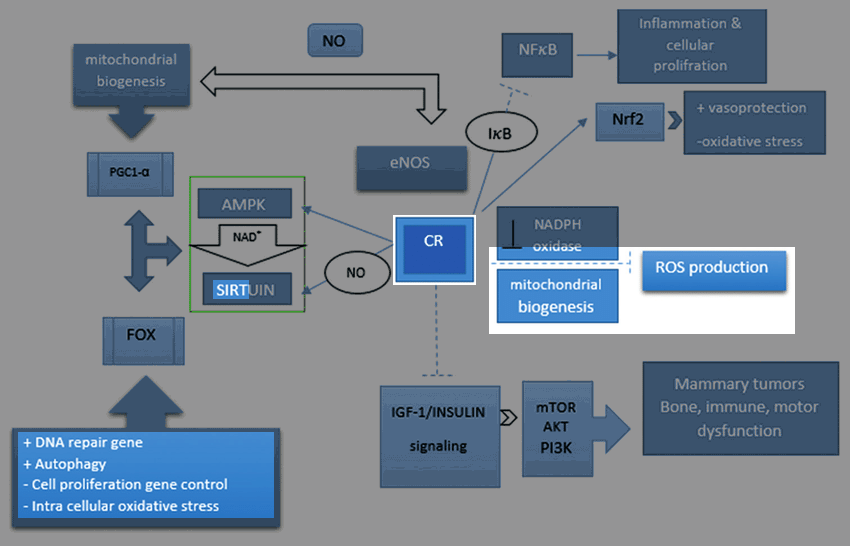
\includegraphics[height=0.85\textheight]{cr_pathways_highlights} \\
    Source: \cite{hanjani2018protein}, highlights added
\end{frame}


\begin{frame}[c]{Calorie Restriction Effects}
    \large
    \begin{itemize}[<+(1)->]
        \item 'Different' mitochondrial energy production (less ROS)
        \item Increased repair capacity (SIRT and others)
        \item Increased removal of misfolded proteins
        \item Reduced intracellular (oxidative) stress
        \item Reduced inflammation and proliferation
    \end{itemize}
    Overall: Optimizing energy and resource usage
\end{frame}


\subsection{Senescent Feedback Loop}

\begin{frame}[c]
    Feedback loop 1: mitochondrial high ROS-state (due to emergency state) and resulting DNA-damage causing prolonged emergency state
    Feedback loop 2: repair pathways fixing dna damage unrestraining transposons proliferating and causing further dna damage
    resulting in SASP
\end{frame}
